\documentclass[conference]{IEEEtran}
\IEEEoverridecommandlockouts
% The preceding line is only needed to identify funding in the first footnote. If that is unneeded, please comment it out.
\usepackage{cite}
\usepackage{amsmath,amssymb,amsfonts}
\usepackage{algorithmic}
\usepackage{graphicx}
\usepackage{textcomp}
\usepackage{xcolor}
\usepackage{longtable}
\usepackage{array}
\usepackage[german]{babel}
\usepackage[utf8x]{inputenc}
\usepackage[german=quotes]{csquotes}
\def\BibTeX{{\rm B\kern-.05em{\sc i\kern-.025em b}\kern-.08em
    T\kern-.1667em\lower.7ex\hbox{E}\kern-.125emX}}
\begin{document}

\title{Random Forest und k-Nearest-Neighbours für die Detektion von Schreibstiländerungen zur Autorenzuordnung}





\author{\IEEEauthorblockN{Engler, Rebecca; Fandrich, Anna; Gühler, Tobias; Mitterlehner, Johanna; Schilling, Anabel;\\ Wittmann, Clarissa; Wutke, Leon}
\IEEEauthorblockA{Fakultät CB} \\
\textit{HS Mittweida}
}
\maketitle

\begin{abstract}
This document is a model and instructions for \LaTeX.
This and the IEEEtran.cls file define the components of your paper [title, text, heads, etc.]. *CRITICAL: Do Not Use Symbols, Special Characters, Footnotes, 
or Math in Paper Title or Abstract.
\end{abstract}

\begin{IEEEkeywords}
	machine learning, text mining, author detection
\end{IEEEkeywords}

\section{Einleitung}
	Style Change Detection ist ein Verfahren, dessen Ziel es ist zu bestimmen, wo in einem gemeinschaftlich geschriebenen Text ein Wechsel des Autors stattfindet \cite{e_b1}. Es überprüft, wie gleichmäßig der Schreibstil im ganzen Text ist und an welchen Stellen er sich ändert, was auf einen Wechsel des Autors hindeutet \cite{e_b2}. Dabei werden verschiedene stilistische Eigenschaften, sogenannte Features, verwendet. Diese werden im ganzen Text miteinander verglichen und überprüft, an welchen Stellen sich wie viele Features wie stark verändern, um einzuschätzen, ob ein Autorenwechsel stattgefunden hat \cite{e_b3}. Das Verfahren kann für verschiedene forensische Zwecke verwendet werden, wie zum Beispiel die Identifizierung von Plagiaten \cite{e_b2}.
	
	Die Aufgabe hierbei besteht darin, in einem Dokument, geschrieben von mehreren Autoren, Änderungen des Schreibstils und der damit verbundene Wechsel des Autors zu erkennen. Dafür wird angenommen, dass der Wechsel des Stils den Wechsel des Autors impliziert. Gegeben sind hierfür englische Dokumente. Diese können bis zu zehn Stiländerungen enthalten und von höchstens drei Verfassern stammen. Gleichzeitig können Änderungen des Stils nur zwischen Absätzen vorkommen, was einen Autor und einen Stil pro Absatz impliziert. Durch diese festgesetzten Bedingungen werden nun die Frage nach der Verfassung des Dokuments durch mehrere Autoren und die Frage nach Stilwechseln zwischen Absätzen bezogen auf jedes aufeinanderfolgende Paar von Absätzen in einem Dokument beantwortet.
	
	Ziel des Projektes ist es anhand eines Programms zu ermitteln, ob die bereitgestellten Dokumente Änderungen des Stils enthalten. Trifft dies zu wird versucht, diese Änderungen im Text zu lokalisieren.
	
	Im Folgenden werden verwandte Werke besprochen. Daraufhin beschäftigt man sich mit den Methoden, bestehend aus Datensatz, Algorithmus und Features. Abschließend werden die Ergebnisse dargelegt, woraufhin die Diskussion und ein Fazit folgen.
	
\section{Verwandte Werke}
Seit dem Jahr 2017 erscheint \textcolor{gray}{\enquote{Style Change Detection}} als Aufgabe des PAN als Teil des CLEFs (Conference and Labs of the Evaluation Forum). Seitdem wurden zahlreiche Vorgehen erprobt, um die Aufgabenstellung zu bewältigen und die bisherigen Ergebnisse zu verbessern. \cite{vw_b1} 

Iyer und Vosoughi \cite{vw_b2} nutzen Googles BERT-Modell für die Erstellung von Worteinbettungen auf Satzebene als Repräsentation der Texte. Mit den Ausgaben aus BERT wird eine Feature-Matrix erstellt, die dann für aufeinanderfolgende Absätze und das gesamte Dokument zusammengefasst wird. Zuletzt erfolgt die Übergabe an einen Random Forest Klassifikator zum Training.

Singh et al. \cite{vw_b3} extrahieren Eigenschaften zweier Absätze und stellen diese als Eigenschaftsvektoren dar. Anhand der Unterschiede dieser zwei Vektoren und eines Klassifikators für Logistische Regression wird die Stiländerungserkennung durchgeführt. 

Deibel und Löfflad \cite{vw_b4} kombinieren Worteinbettungen mit bekannten stilometrischen Eigenschaften. Sie nutzen ein Multi-Layer-Perceptron zur Erkennung multipler Autoren im Dokument und ein bidirektionales „Long short-term memory“ (LSTM) zur Erkennung der Stiländerung. Der Ansatz iteriert nachfolgend und teilt unter Zuhilfenahme eines Attribution-Algorithmuses einen Autor pro Absatz zu.

Viele der bisherigen Vorgehen extrahieren stilometrische Eigenschaften aus den vorgegebenen Textdaten und nutzen diese, um Ähnlichkeit zwischen den Absätzen festzustellen \cite{vw_b5,vw_b6,vw_b7}. Der in der vorliegenden Arbeit verwendete Ansatz ähnelt diesem Muster. Unterschiede sind unter Anderem bei der Verarbeitung der Features anzumerken. 

Wie Deibel und Löfflad \cite[S.9]{vw_b4} in ihrer Arbeit anmerken, scheint die Auswahl der verwendeten Features großen Einfluss auf das Endergebnis der Style-Change-Detection-Aufgabe zu haben. So erzielten sie auch mit lediglich fünf Eigenschaften gute Ergebnisse auf dem in ihrer Arbeit verwendeten Datensatz.  

In der vorliegenden Arbeit wurde hier angesetzt und nur Features verwendet, die aussagekräftig für die Problemlösung waren. 

Singh et al \cite[S.4]{vw_b8} diskutieren die Problematik, dass extrahierte Eigenschaften bei kurzen Dokumenten- bzw. Absatzlängen weniger relevante stilometrische Information böten. Sie nutzten daher kompakte Feature-Sets, die mit dem Stil zusammenhängende Feature über das gesamte Dokument sammeln.
 
Der in der vorliegenden Arbeit verwendete Lösungsansatz ist die Gewichtung der Features abhängig von der Länge des Absatzes. 

Neben der Verwendung bekannter stilometrischer Eigenschaften wurden in verwandten Werken auch Worteinbettungen als textuelle Eigenschaften auf Wort- \cite{vw_b9} und Satzebene \cite{vw_b2} zur Autorenzuordnung eingesetzt. Auf die Nutzung dieser wird bei der vorliegenden Arbeit verzichtet.

Ein weiterer Unterschied des hier vorgelegten Ansatzes zu vorherigen Arbeiten ist ein neues Vorgehen für den Random Forest Klassifikator, auf das im Abschnitt X noch näher eingegangen wird.

\section{Methoden}
	\subsection{Datensatz}
		Zur Lösung des in der Einleitung beschriebenen Problems liegen ein Traningsdatensatz sowie ein Validierungsdatensatz vor. Weiterhin sind beide Datensätze unterteilt in je einen wide sowie einen narrow Datensatz. Der narrow Datensatz ist auf einen kleinen Themenbereich beschränkt während der wide Datensatz einen größeren Themenbereich umfasst. Die Anzahl der Dokumente, die in jedem der Datensätze enthalten sind, lässt sich aus Tabelle \ref{tab:ds_1} entnehmen.
		\begin{table}[htbp]
			\caption{Anzahl der Dokumente pro Datensatz}
			\begin{center}
				\begin{tabular}{|c|c|c|}
					\hline
					& Narrow & Wide \\
					\hline 
					Training & 3442 & 8138 \\
					\hline
					Validation & 1722 & 4078 \\
					\hline 
				\end{tabular}
				\label{tab:ds_1}
			\end{center}
		\end{table}
	
	
		Für die gegebenen Daten wurde zunächst eine Datenexploration ausgeführt, um deren Struktur zu analysieren. Hierbei wurde anfangs die Verteilung der Autoren über die Dokumente des Trainingsdatensatz betrachtet. Es ergab sich das 4024 Dokumente von einem Autor geschrieben wurden, 1990 Dokumente zwei Autoren haben sowie 2015 von drei Autoren geschrieben wurden.
		
		Im nächsten Schritt wurde analysiert, ob die Dokument Code enthalten, welcher bei der Erstellung der Dokumente mit aus den Stackoverflow Seiten extrahiert wurde. Der gefundene Code wurde dann entfernt, da dieser Code, aufgrund der vorgegebenen Syntaktik, meist andere autorspezifische Merkmale aufweist als natürliche Sprache (in Textform).
		Obwohl vorgegeben war das alle Dokumente in englischer Sprache verfasst wurden, wurde als letztes die Sprache der gegebenen Dokumente untersucht, um anderssprachige Dokumente aus dem Datensatz auszuschließen. Dabei wurden Bruchstücke deutscher Sprache und Sprachen aus dem asiatischen Raum gefunden.
		
\subsection{Algorithmus}
	Für Aufgabe 2, also um zu erkennen, welcher Autor den jeweiligen Absatz geschrieben hat, wird ein Random Forest Klassifikator mit verschiedenen Features genutzt. Für den Klassifikator wird die scikit-learn Bibliothek für Python verwendet \cite{ma_b1}. Die verwendeten Features sind in Tabelle \ref{tab:features} aufgeführt. Diese Features werden über jeden einzelnen Absatz berechnet. Diese Ergebnisse werden dann an den Random Forest-Klassifikator weitergegeben, der die Absätze dann wie unten bzw. in Abbildung \ref{fig:algorithm} erklärt den Autoren zuordnet.
	
	Random Forests haben einige Vorteile, die für die Aufgabe nützlich sind. Unter anderem, sind Training sowie Voraussage schnell. Der Algorithmus kann zudem parallel implementiert werden und ist für hochdimensionale Probleme – wie Style Change Detection – geeignet. \cite{ma_b2} Außerdem nutzt er nicht alle Daten, sodass ein ausreichend großer Evaluationsdatensatz vorhanden ist.
	
	Die Anzahl solcher Entscheidungsbäume kann variieren. Es hat sich aber gezeigt, dass eine höhere Anzahl an Bäumen nicht zwingend bessere Ergebnisse liefert. Da der Random Forest mehrere Entscheidungsbäume auf einmal verwendet ist auch die Gefahr des Overfittings reduziert. \cite{ma_b2}
	
	\begin{figure}[h]
		\centering
		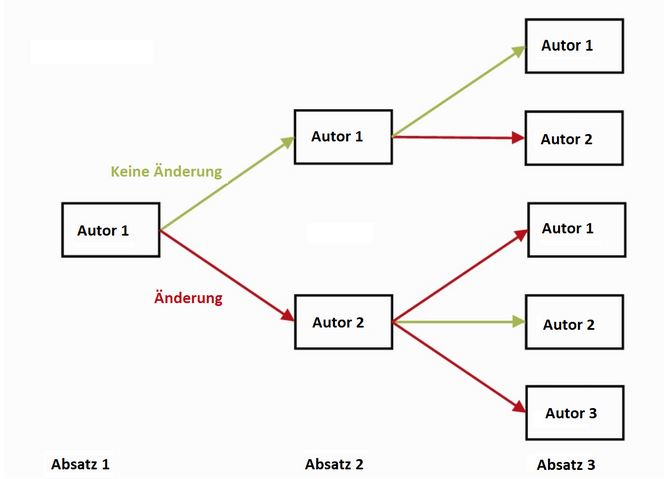
\includegraphics[width=0.7\linewidth]{../../Unbenannt}
		\caption{Grafische Darstellung des Random Forest-Klassifikator}
		\label{fig:algorithm}
	\end{figure}
	
	
	Da ein Autorenwechseln nur zwischen den Absätzen stattfindet, kann angenommen werden, dass der erste Absatz von Autor 1 geschrieben wurde. Wird eine Änderung zu Absatz 2 festgestellt, dann wurde dieser Absatz von einem anderen Autor (Autor 2) geschrieben, andernfalls wurde auch dieser Absatz von Autor 1 geschrieben. Das wird durch das gesamte Dokument fortgeführt, wobei der dritte Absatz auch von Autor 3  geschrieben worden sein kann. Die Voraussetzung ist allerdings, dass es in Absatz 2 einen Autorenwechsel von Autor 1 zu Autor 2 gibt. Um einen dritten Autor festzustellen werden beispielsweise Absatz 1 und Absatz 3 miteinander verglichen, um zu bestimmen, ob zwischen diesen beiden Absätzen ein Autorenwechsel stattgefunden hat. Wenn es eine Änderung gab wurde Absatz 3 von Autor 3 geschrieben, ansonsten wieder von Autor 1. Das kann man Abbildung 1 entnehmen. 
	.
	Zuletzt wird das mittlere Featureset der einzelnen Autoren bestimmt. Dadurch kann in einem anderen Dokument eindeutig beurteilt werden, ob ein Autor in beiden Dokumenten geschrieben hat. Da z.B. Autor 1 in Dokument 1 auch Autor 2 in Dokument 2 sein kann ist es notwendig diese Werte zu berechnen und anschließend zu vergleichen.
	
\subsection{Features}
	Autoren können anhand von stilometrischen Featuren unterschieden werden. Es gibt vier Arten von Features: lexikalische, syntaktische, strukturelle und inhaltsbasierte. In Tabelle \ref{tab:features} ist eine Auswahl der verwendeten Features gelistet. Es wurden hauptsächlich lexikalische Features verwendet, da sie zeigen, welche Satzzeichen und Wörter Autoren unabhängig von anderen Faktoren verwenden \cite{mf_b1}.
	 
	Um eine allgemeine Unterscheidung von Autoren zu erhalten sollte der Ansatz nicht auf inhaltsbasierten Features aufbauen, da der Gebrauch der Wörter meist vom Inhalt abhängt und somit je nach Inhalt eines Textes stark variiert. Diese Features sind für die gegebene Aufgabe nicht optimal und weitestgehend unbrauchbar \cite{mf_b2}.
	Außerdem eignen stilometrische Features sich gut für längere Texte anstelle von kurzen Nachrichten wie z.B. Tweets und sind somit gut für das gegebene Datenset geeignet \cite{mf_b3}.
	
	Nachfolgend wird eine Auswahl der Features aus Tabelle \ref{tab:features} erklärt.
	Ein wichtiges Feature ist der Flesch Reading Ease. Diese Formel berechnet die Lesbarkeit des Textes und bestimmt somit die Schulbildung, die der Autor benötigt hat, um den Text zu schreiben. Sie hängt von verschiedenen Faktoren ab:
	
	
	$RE = 206.835 - 84.6*WL - 1.015*SL$
	
	
	
	$WL$ repräsentiert hierbei die durchschnittliche Wortlänge in Silben, $SL$ die durchschnittliche Satzlänge. Die in der Formel vorkommenden Zahlen basieren auf Erkenntnissen der Lesbarkeitsforschung und den statistischen Häufigkeiten von Silbenlänge, Wortlänge und Satzlänge im Englischen \cite{mf_b4}.
	Die Anzahl an Füllwörtern ist ebenfalls ein diskriminierendes Feature, da die Anzahl an Synsemantika je nach Autor zwischen 150 und 675 verschiedenen Wörtern liegen kann. Synsemantika sind Wörter mit geringer inhaltlicher Bedeutung, die aber grammatikalisch wichtig sind. Ein Beispiel wäre das Wort ‘dieser’ \cite{mf_b5}.
	
	\begin{table}[htbp]
		\caption{genutzte Features}
		\begin{center}
			\begin{tabular}{|c|c|}
				\hline
				\textbf{Feature} & \textbf{Art} \\
				\hline 
				absolute Zahl an Wörtern & Lexikalisch (Wortbasiert) \\
				\hline
				relative Anzahl an kurzen Wörtern \\ (1-3 Zeichen lang) (relativ zur absatzlänge) & Lexikalisch \\
				\hline 
				Relative Satzlänge (Relativ zur Satzanzahl) & Lexikalisch \\
				\hline
				Durchschnittliche Wortlänge & Lexikalisch \\
				\hline
				Durchschnittliche Wortzahl pro Satz & \\
				\hline
				Absolute Satzzahl & \\
				\hline
				Satzkomplexität & \\
				\hline
				Durchschnittliche Silbenzahl pro Wort & \\
				\hline
				Wortvarianz & Lexikalisch \\
				\hline
				Flesch Reading Ease & Lexikalisch \\
				\hline
				relative Anzahl an Abkürzungen mit \grq \\(relativ zur absatzlänge) & \\
				\hline 
				Sprache \cite{mf_b6} & \\
				\hline
				relative Zahl Sonderzeichen & \\
				\hline
				relative Zahl Füllwörter & \\
				\hline
			\end{tabular}
			\label{tab:features}
		\end{center}
	\end{table}
\section{Ergebnisse}
\section{Diskussion}
\section{Fazit}


\begin{thebibliography}{00}
\bibitem{e_b1} E. Zangerle, M. Tschuggnall, G. Specht, M. Potthast, B. Stein, Overview of the Style Change Detection Task at PAN 2019, in: L. Cappellato, N. Ferro, D. Losada, H. Müller (Eds.), CLEF 2019 Labs and Workshops, Notebook Papers, CEUR-WS.org, 2019.
\bibitem{e_b2} Nath, S. (2021).  Style change detection using Siames neural networks.
\bibitem{e_b3} E. Dauber, R. Overdorf, R. Greenstadt, Stylometric Authorship Attribution of Collaborative Documents, in: S. Dolev, S. Lodha (Eds.), Cyber Security Cryptography and Machine Learning - First International Conference, CSCML 2017, Proceedings, volume 10332 of Lecture Notes in Computer Science, Springer, 2017, S. 115–135.
\bibitem{vw_b1} Pan Webis Group (2021). Shared Tasks. PAN.
\bibitem{vw_b2} A. Iyer and S. Vosoughi. Style Change Detection Using BERT—Notebook for PAN at CLEF 2020. In Linda Cappellato, Carsten Eickhoff, Nicola Ferro, and Aurélie Névéol, editors, CLEF 2020 Labs and Workshops, Notebook Papers, September 2020. CEUR-WS.org.
\bibitem{vw_b3} J. Weerasinghe, R. Singh, and R. Greenstadt. Feature Vector Difference based Authorship Verification for Open-World Settings—Notebook for PAN at CLEF 2021. In Guglielmo Faggioli et al., editors, CLEF 2021 Labs and Workshops, Notebook Papers, September 2021. CEUR-WS.org.
\bibitem{vw_b4} R. Deibel and D. Löfflad. Style Change Detection on Real-World Data using an LSTM-powered Attribution Algorithm—Notebook for PAN at CLEF 2021. In Guglielmo Faggioli et al., editors, CLEF 2021 Labs and Workshops, Notebook Papers, September 2021. CEUR-WS.org.
\bibitem{vw_b5} D. Castro-Castro, C. Alberto Rodríguez-Losada, and R. Muñoz. Mixed Style Feature Representation and B0-maximal Clustering for Style Change Detection—Notebook for PAN at CLEF 2020. In Linda Cappellato, Carsten Eickhoff, Nicola Ferro, and Aurélie Névéol, editors, CLEF 2020 Labs and Workshops, Notebook Papers, September 2020. CEUR-WS.org.
\bibitem{vw_b6} E. Zangerle, M. Tschuggnall, G. Specht, M. Potthast, B. Stein. Overview of the Style Change Detection Task at PAN 2019. In L. Cappellato, N. Ferro, D. Losada, H. Müller (Eds.), CLEF 2019 Labs and Workshops, Notebook Papers, 2019. CEUR-WS.org,
\bibitem{vw_b7} E. Dauber, R. Overdorf, R. Greenstadt. Stylometric Authorship Attribution of Collaborative Documents. In S. Dolev, S. Lodha (Eds.), Cyber Security Cryptography and Machine Learning - First International Conference, CSCML 2017, Proceedings, volume 10332 of Lecture Notes in Computer Science, Springer, 2017, S. 115–135.
\bibitem{vw_b8} R. Singh, J. Weerasinghe, and R. Greenstadt. Writing Style Change Detection on Multi-Author Documents—Notebook for PAN at CLEF 2021. In Guglielmo Faggioli et al., editors, CLEF 2021 Labs and Workshops, Notebook Papers, September 2021. CEUR-WS.org.
\bibitem{vw_b9} K. Safin and R. Kuznetsova. Style Breach Detection with Neural Sentence Embeddings—Notebook for PAN at CLEF 2017. In Linda Cappellato, Nicola Ferro, Lorraine Goeuriot, and Thomas Mandl, editors, CLEF 2017 Evaluation Labs and Workshop – Working Notes Papers, 11-14 September, Dublin, Ireland, September 2017. CEUR-WS.org.
\bibitem{ma_b1} https://scikit-learn.org
\bibitem{ma_b2} Cutler, Cutler, Stevens. Random Forests. Ensemble Machine Learning, pp.157-176. 2012.
\bibitem{mf_b1} S. Elmanarelbouanani and I. Kassou. Authorship Analysis Studies: A Survey. International Journal of Computer Applications, 86, 2013.
\bibitem{mf_b2} R. Zheng and J. Li and H. Chen and Z. Huang. A framework for authorship identification of online messages: Writing-style features and classification techniques. Journal of the American Society for Information Science and Technology, 57(3), 378–393, 2006. doi:10.1002/asi.20316.
\bibitem{mf_b3} B. Stein and N. Lipka and P. Prettenhofer. Intrinsic plagiarism analysis. Lang Resources and Evaluation 45, 63–82, 2011. https://doi.org/10.1007/s10579-010-9115-y.
\bibitem{mf_b4} Bailin, Grafstein. Readability: Text and Context, pp. 35-38, 2016.
\bibitem{mf_b5} https://www.duden.de/rechtschreibung/Synsemantikon
\bibitem{mf_b6} https://pypi.org/project/langdetect/
\end{thebibliography}

\end{document}
